Para alcanzar los objetivos planteados, es necesario abordar una serie de temas claves que proporcionarán contexto y comprensión técnica necesarios para desarrollar el proyecto. 

\subsection*{Crazyflie 2.1 }
Los drones Crazyflie son plataformas de desarrollo aéreo de código abierto desarrollados por Bitcraze. Están diseñados principalmente para investigación, desarrollo y educación en ingeniería de control y robótica. Como se observa en la Figura \ref{fig:Crazyflie}, tienen un tamaño reducido, pero están equipados con una variedad de sensores que lo vuelven ideal para explorar algoritmos de control y otras aplicaciones. 
\begin{figure}[htbp]
	\centering
	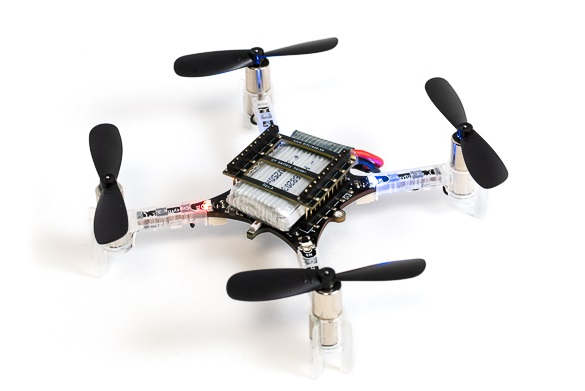
\includegraphics[width=0.45\textwidth]{Crazyflie}
	\caption{Dron Crazyflie 2.1 \cite{Crazyflie}.}
	\label{fig:Crazyflie}
\end{figure}
\\El Crazyflie 2.1 es un mini dron que pesa aproximadamente 27 gramos y tiene dimensiones generales de 92mm x 92mm x 29mm. Su control se realiza mediante Bluetooth o radiofrecuencia, lo que le permite ser controlado desde dispositivos móviles, así como desde sistemas operativos Windows, Mac OSX y Linux utilizando Crazyradio o Crazyradio PA. En cuanto a sus características eléctricas, el Crazyflie 2.1 dispone de una batería de litio-polímero (Li-Po) con modos desde 100 mA hasta 980 mA, que alimenta motores, microcontroladores y demás componentes. Utiliza un microcontrolador STM32F405 para el control de vuelo y un microcontrolador nRF51 para la comunicación inalámbrica. Está equipado con un acelerómetro/giroscopio de 3 ejes BMI088 y un sensor de presión de alta precisión BMP388, pero también permite la integración de otras placas de expansión para ampliar sus capacidades, con la restricción de que soporta una carga adicional de hasta 15 gramos que puede afectar el tiempo de vuelo debido al aumento de demanda de energía \cite{Crazyflie}. 

\subsection*{Sistema de coordenadas de drones Crazyflie}
Los drones Crazyflie, al igual que la mayoría de los drones, utilizan la convención de sistema de coordenadas tridimensional ENU (East North Up) para determinar su posición y orientación en el espacio. Como se observa en la Figura \ref{fig:Sistema_Crazyflie}, el dron tiene tres ejes principales de referencia: el eje X es horizontal y apunta hacia adelante, el eje Y es horizontal y apunta hacia la derecha y el eje Z es vertical y apunta hacia arriba. 

Por otro lado, la orientación del dron se describe en términos de ángulos de inclinación respecto a los ejes de referencia. El ángulo de balanceo (roll) se refiere a la inclinación del dron hacia los lados en torno al eje X, el ángulo de cabeceo (pitch) se refiere a la inclinación hacia adelante o hacia atrás en torno al eje Y, y el ángulo de guiñada (yaw) se refiere a la rotación del dron en torno al eje Z. Según la documentación oficial de Bitcraze, estos ángulos siguen las siguientes reglas de rotación: roll y yaw rotan en sentido horario alrededor del eje al mirar desde el origen, mientras que pitch rota en sentido antihorario alrededor del eje al mirar desde el origen \cite{Sistema_Crazyflie}.

\begin{figure}[htbp]
	\centering
	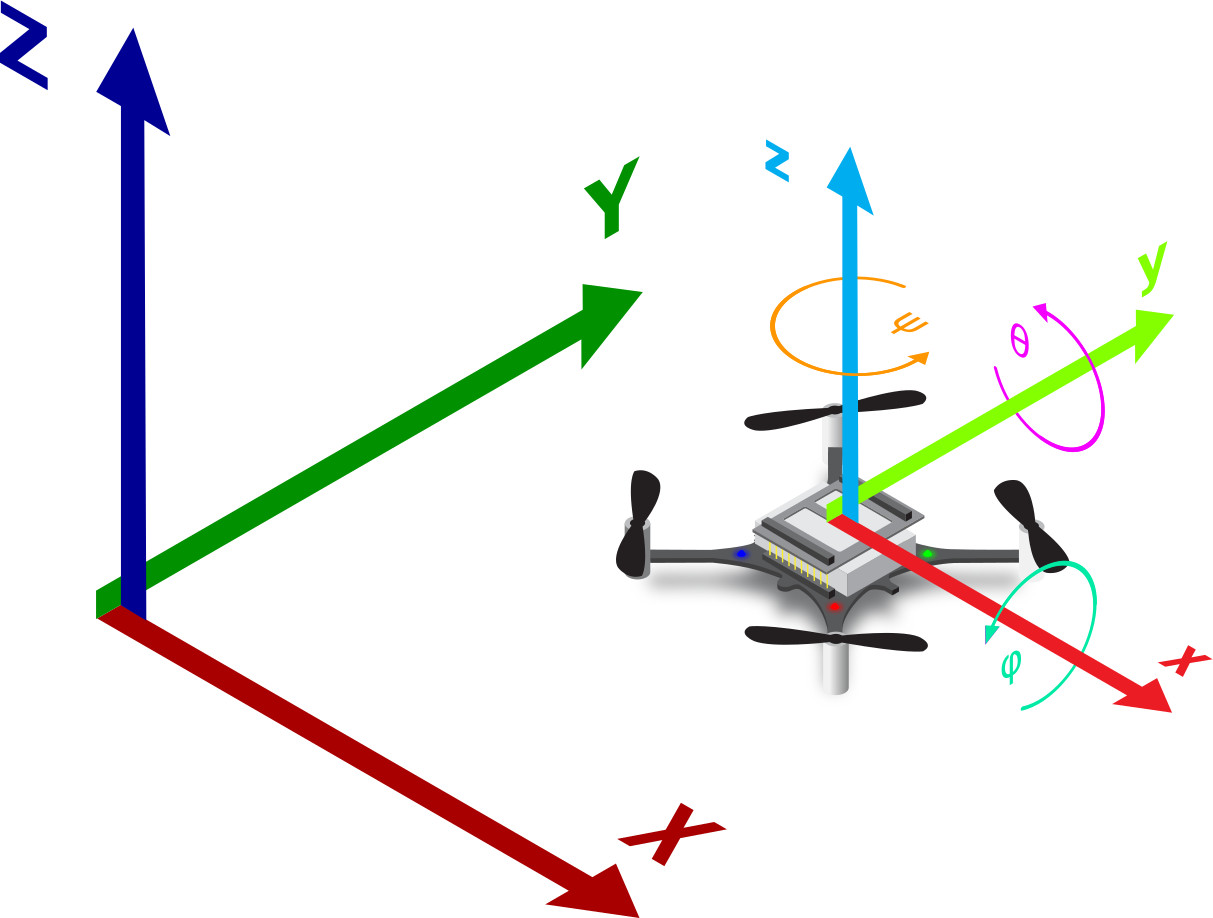
\includegraphics[width=0.6\textwidth]{Sistema_Crazyflie}
	\caption{Sistema de coordenadas de Crazyflie 2.1 \cite{Sistema_Crazyflie}.}
	\label{fig:Sistema_Crazyflie}
\end{figure}

\subsection*{Comunicación inalámbrica de drones Crazyflie}
Los drones Crazyflie establecen una comunicación inalámbrica por medio del dispositivo Crazyradio, mostrado en la Figura \ref{fig:Crazyradio}. Esta comunicación se basa en un enlace de radiofrecuencia bidireccional que permite enviar comandos de control al dron y recibir datos en tiempo real sobre su posición, orientación y otros parámetros relevantes.   
\begin{figure}[htbp]
	\centering
	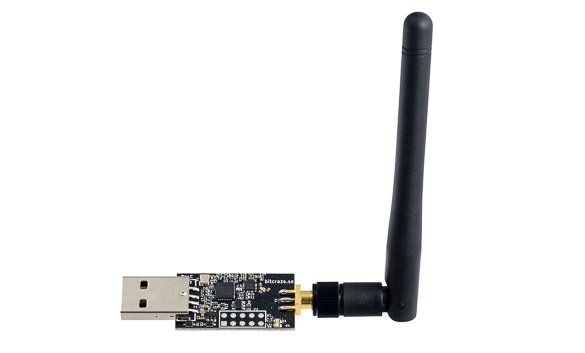
\includegraphics[width=0.4\textwidth]{Crazyradio}
	\caption{Dispositivo de comunicación inalámbrica Crazyradio \cite{Crazyradio}.}
	\label{fig:Crazyradio}
\end{figure}
\\ El Crazyradio es un transceptor de radio USB de código abierto, baja latencia y largo alcance. Funciona en la banda de 2.4 GHz con un rango de transmisión de hasta 1 km (en condiciones ideales) gracias a su amplificador de radio de 20 dBm. Está basado en el microcontrolador nRF24LU1 de Nordic Semiconductor y se comunica por medio del protocolo “Enhanced ShockBurst” compatible con los microcontroladores nRF24L01p, nRF51 y nRF52. En una capa de nivel más alto, utiliza el protocolo de paquetes CRTP para comunicarse con el Crazyflie y poder actualizar el firmware, enviar comandos y recibir información de los drones. Dependiendo del sistema operativo, es necesario instalar controladores o realizar configuraciones específicas \cite{Crazyradio}.

\subsection*{Flow Deck}
El Flow Deck es una placa de expansión para el dron Crazyflie y que le otorga la capacidad de comprender su movimiento en cualquier dirección. Utiliza un medición de distancias VL53L1x para determinar su altura junto a un sensor de flujo óptico PMW3901 que mide movimientos horizontales sobre la superficie por medio de odometría visual.  La placa de expansión Flow Deck, mostrada en la Figura \ref{fig:FlowDeck}, tiene un peso aproximado de 1,6 gramos y dimensiones generales de 21mm x 28mm x 4mm. Para integrarlo se requiere actualizar el firmware del Crazyflie a su última versión y montarlo en la parte inferior del dron. \cite{FlowDeck}. 
\begin{figure}[htbp]
	\centering
	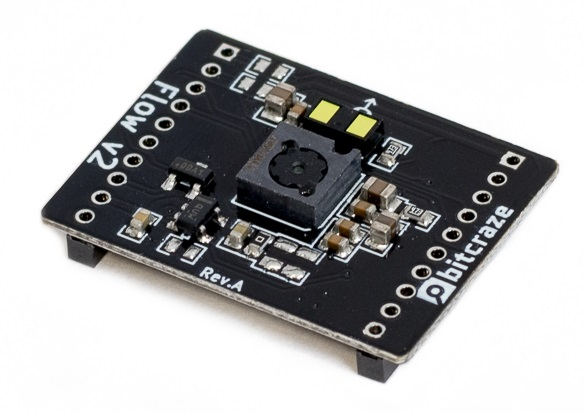
\includegraphics[width=0.35\textwidth]{FlowDeck}
	\caption{Placa de expansión Flow Deck v2 \cite{FlowDeck}.}
	\label{fig:FlowDeck}
\end{figure}
\subsection*{Odometría visual}
La odometría visual es un proceso mediante el cual se utiliza información extraída de imágenes para estimar el movimiento, en este caso relacionado con un vehículo o robot. En esta técnica de estimación de posición se emplea una secuencia de imágenes para calcular la trayectoria de rasgos visuales distintivos en las imágenes y el análisis de cómo estos cambian entre imágenes consecutivas. Los sistemas de odometría visual son capaces de generar un mapa tridimensional del entorno y un registro de la trayectoria para determinar la localización del agente. En esencia, la odometría visual se basa en la geometría de las imágenes capturadas por cámaras, utilizando algoritmos para minimizar la proyección repetitiva de puntos tridimensionales a partir de las características visuales coincidentes entre imágenes \cite{Persson2022_book}. 
\begin{figure}[htbp]
	\centering
	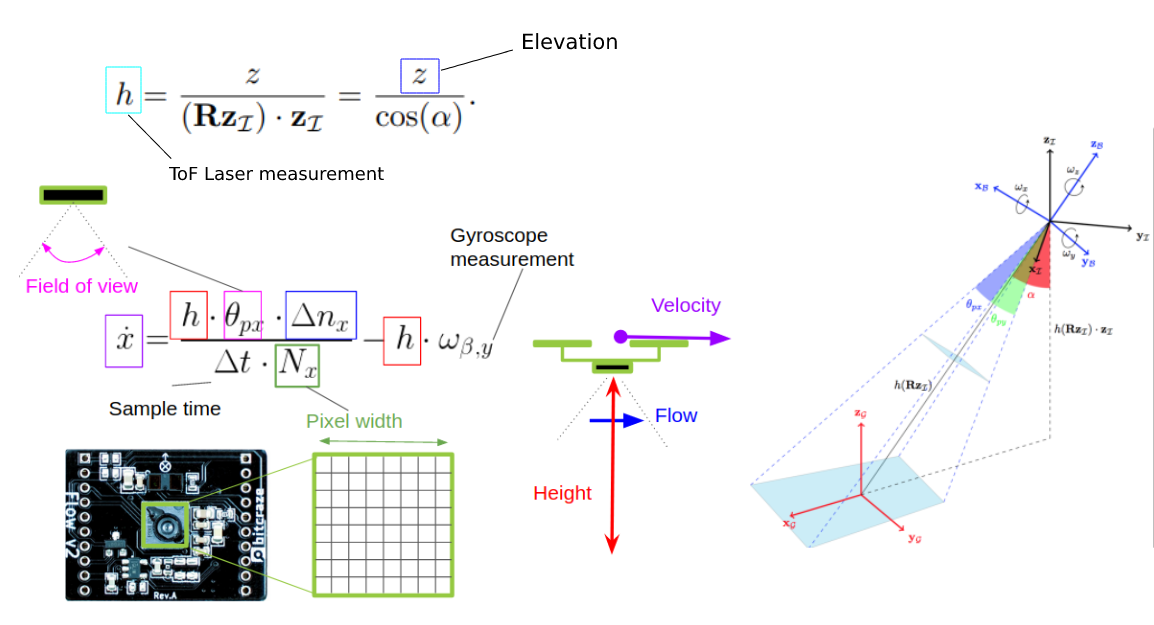
\includegraphics[width=0.7\textwidth]{Funcionamiento_FlowDeck}
	\caption{Gráfico de funcionamiento de Flow Deck \cite{Funcionamiento_FlowDeck}.}
	\label{fig:Funcionamiento_FlowDeck}
\end{figure}
\\Como se mencionó con anterioridad y justo como se evidencia en la Figura \ref{fig:Funcionamiento_FlowDeck}, el Flow Deck utiliza odometría visual para obtener las mediciones de posición en el plano horizontal. Esta información se combina con las mediciones del sensor de distancia para determinar la posición del Crazyflie en relación con su entorno. \cite{Funcionamiento_FlowDeck}.

 \subsection*{Sensor de flujo óptico PMW3901}
El PMW3901 es un sensor de flujo óptico desarrollado por Pixart Imaging, ampliamente utilizado en aplicaciones de robótica para medir movimiento. Resulta de particular interés debido a que forma parte de la placa de expansión Flow Deck de Bitcraze y es el responsable de darle sentido de posición bidimensional (en los ejes X-Y) a los drones Crazyflie. Dentro de sus detalles técnicos, dispone un microcontrolador de bajo consumo que determina internamente el flujo óptico con algoritmos de odometría visual, proporcionando posición con base en diferencias en pixeles entre fotogramas. Opera con un voltaje que varía entre 1.8 y 2.1V. Se comunica por medio de una interfaz SPI de 4 hilos que opera a 2 MHz, transmitiendo datos de movimiento almacenados en registros de 16 bits. Tiene un rango de operación desde 80 mm hasta el infinito y cuenta con una tasa de fotogramas de 121 FPS, detectando movimientos de hasta 7.4 radianes por segundo. Finalmente, está encapsulado en un paquete chip-on-board de 28 pines, lo que permite su integración en distintas aplicaciones \cite{PMW3901_datasheet}.

\subsection*{Sensor de medición de distancias VL53L1x}
El VL53L1x es un sensor de medición de distancias desarrollado por STM electronics. La placa de expansión Flow Deck tiene integrado este sensor para proporcionar sentido de altura de vuelo (eje Z) a los drones Crazyflie. En cuanto a sus especificaciones técnicas, el VL53L1x está basado en la tecnología de tiempo de vuelo (Time-of-Flight, ToF) que permite medir el tiempo que tarde un pulso de luz en reflejarse desde un objeto y volver al sensor, proporcionando una medida precisa de la distancia del objeto. El sensor funciona emitiendo un láser invisible de 940 nm y utiliza una matriz de recepción SPAD (diodo de avalancha de fotón único) para detectar la luz reflejada, ofreciendo un campo de visión típico de 27 grados. Incluye un microcontrolador de bajo consumo que permite una medición de distancia de hasta 4 metros con una frecuencia de hasta 50 Hz y se comunica por medio de una interfaz I2C que soporta velocidades de hasta 400 kHz \cite{VL53L1x_datasheet}.

\subsection*{Librería en Python para Crazyflie}
Existe una librería en Python desarrollada por el grupo Bitcraze cuya función es simplificar el uso y control de los drones Crazyflie. Esta librería disponde de funciones de alto nivel que facilitan la conexión, registro de datos, envío de comandos y manipulación de parámteros del dron. Está diseñada para ser utilizada con los drones Crazyflie por medio del dispositivo Crazyradio, admitiendo enlaces de comunicación mediante diferentes interfases tales como radio, USB, serial, entre otras. Dentro de las funciones de alto nivel que presenta, están algunas para envío de comandos de control de actitud y posición, así como otras para configuración de registros y monitoreo de variables del firmware en tiempo real \cite{Crazyflie_Python}. 

\subsection*{Protocolo de comunicación CRTP}
CRTP es el protocolo de empaquetamiento de datos utilizado para comunicarse con los drones Crazyflie. Este protocolo estructura los paquetes de información para dirigirlos a funcionalidades específicas del dron como el registro de datos, control de movimiento y parámetros de configuración \cite{Crazyflie_CRTP}. 

\subsubsection*{Pila de comunicación}
La comunicación con Crazyflie se implementa como una pila de capas independientes. En la base se encuentra el medio físico (radio o USB), seguido por el enlace que garantiza la transmisión segura y ordenada de paquetes. Encima de esto está CRTP que maneja información de puerto y canal para dirigir los paquetes de datos a los distintos subsistemas del Crazyflie. Por último, los subsistemas implementan las funcionalidades del dron, controladas a través de CRTP.

\subsubsection*{Implementación de enlaces}
Existen dos implementaciones de enlace activamente soportadas para Crazyflie: el enlace de radio, que utiliza radios compatibles con nRF24, y el enlace USB, que se conecta directamente al puerto USB del Crazyflie. Cada uno de estos enlaces asegura la transmisión ordenada y segura de paquetes entre el controlador y el dron.

\subsubsection*{Ordenación de paquetes y soporte en tiempo real}
CRTP (Crazy RealTime Protocol) prioriza los paquetes para facilitar el control en tiempo real del Crazyflie. El enlace garantiza el orden estricto de los paquetes dentro de un mismo puerto, aunque los paquetes de diferentes puertos pueden enviarse fuera de orden. La priorización se logra asignando mayor prioridad a los números de puerto más bajos, permitiendo la transmisión simultánea de datos en tiempo real y la carga de trayectorias.

\subsubsection*{Metadatos del paquete CRTP}
Cada paquete CRTP incluye un número de puerto, un número de canal y una carga útil. Los puertos oscilan entre 0 y 15 y los canales entre 0 y 3, con la carga útil limitada a 31 bytes. Estos metadatos permiten dirigir los paquetes a los subsistemas correctos y las funcionalidades específicas dentro del Crazyflie.

\subsubsection*{Paquetes especiales}
El paquete 15:3 es un caso especial denominado null packet, que es ignorado por el Crazyflie y las bibliotecas CRTP. Los null packets se usan para solicitar datos descendentes cuando no hay datos para enviar. También se utilizan para comunicar paquetes fuera del flujo de datos principal, como los paquetes de bootloader, interpretados por el chip de radio nRF51 del Crazyflie.

\subsubsection*{Asignación de puertos}
Los puertos CRTP se asignan a distintos subsistemas en el Crazyflie, permitiendo la comunicación bidireccional entre un subsistema específico y su manejador en tierra. Por ejemplo, el puerto 0 se utiliza para leer el texto de la consola, el puerto 2 para obtener y establecer parámetros, y el puerto 3 para enviar puntos de control de movimiento.

\subsubsection*{Procedimiento de conexión}
Generalmente, CRTP es sin conexión y la mayoría de los subsistemas del Crazyflie intentan ser sin estado. Sin embargo, algunos enlaces y subsistemas mantienen estados específicos, como el enlace USB que necesita ser habilitado mediante un paquete de control USB, y el enlace de radio que utiliza contadores de paquetes para evitar pérdidas y garantizar el orden. La conexión típica incluye inicializar el enlace y los subsistemas soportados, asegurando la transmisión de datos correcta y segura.